\chapter{Suporte Ferramental para Minerar Padr\~{o}es de Uso de Constru\c c\~{o}es da Linguagem Java}

Com o intuito de obter uma compreens\~{a}o sobre o uso 
das constru\c c\~{o}es da linguagem Java, tornou-se 
necess\'{a}ria a implementa\c c\~{a}o de uma ferramenta 
de an\'{a}lise est\'{a}tica de prop\'{o}sito bem 
espec\'{i}fico, por outro lado com capacidade de 
ser extens\'{i}vel para extrair diferentes tipos de 
informa\c c\~{o}es. 
A Figura~\ref{fig:Arquitetura} apresenta 
uma vis\~{a}o geral dos elementos que comp\~{o}em o 
analisador est\'{a}tico desenvolvido durante a condu\c c\~{a}o 
deste trabalho de gradua\c c\~{a}o. Em linhas 
gerais, tal suporte ferramental recupera do sistema 
de arquivos todos os arquivos contendo código fonte 
escrito na linguagem Java, realiza o \textit{parse} 
desses arquivos gerando uma representação 
intermediária correspondente, mais adequada para 
as an\'{a}lises de interesse deste projeto, 
aplica uma série de mecanismos de análise estática 
para coletar as informações sobre o uso das 
caracter\'{i}sticas da linguagem de programa\c c\~{a}o e, por fim, 
gera os resultados no formato 
apropriado para as an\'{a}lises estat\'{i}sticas 
(no contexto deste projeto, foi feita a op\c c\~{a}o pelo 
formato CVS).

Atualmente existem diversas ferramentas e bibliotecas 
de programa\c c\~{a}o que auxiliam a constru\c c\~{a}o
de analisadores estáticos,  
conforme as nossas necessidades.
Entretanto, devido a maior experiência dos 
participantes do projeto com uso da linguagem Java, 
foi feita a op\c c\~{a}o por se utilizar a 
infraestrutura da plataforma \textit{Eclipse Java Development Tools}~\cite{EclipseJDT} 
(Eclipse JDT). O Eclipse JDT 
fornece um conjunto de ferramentas que auxiliam na constru\c c\~{a}o 
de ferramentas que permitem processar c\'{o}digo fonte escrito 
na linguagem de programa\c c\~{a}o Java. 
A plataforma Eclipse JDT é composta por 4 componentes principais: 
APT, \textit{Core}, \textit{Debug} e UI. Neste projeto a 
plataforma foi usada essencialmente através do \textit{JDT Core}, 
que dispõe de uma representa\c c\~{a}o Java 
para a navega\c c\~{a}o 
e manipula\c c\~{a}o dos elementos de uma árvore 
sintática~\acs{AST} gerada a partir do c\'{o}digo fonte, onde os elementos 
da representa\c c\~{a}o correspondem \`{a}s constru\c c\~{o}es 
sint\'{a}ticas da linguagem (como pacotes, classes, interfaces métodos e atributos). 

A~\acs{AST} provida pelo \acs{JDT} é composta por 122 classes, 
como por exemplo existem 22 classe para representar senten\c cas  
como \textit{IF-Than-Else, Switch, While, BreakStatement} 
entre outras. Exitem cinco classes que trabalham exclusivamente com métodos referenciados 
e seis classes exclusivas que tratam os tipos declarados, como classes, interfaces 
e enumera\c c\~{o}es em Java.
O Eclipse JDT~\cite{EclipseJDT} disponibiliza ainda um \textit{parser} 
para a linguagem Java que atende a especifica\c c\~{a}o 
Java 8 da linguagem e que produz a representação intermediária baseada no conjunto de classes Java 
mencionado anteriormente e que corresponde 
a uma~\acs{AST} do código fonte. A plataforma tamb\'{e}m oferece 
uma hierarquia de classes 
para travessia na AST, de acordo com o padr\~{a}o de projeto \textit{visitor}~\cite{Gamma:1995}, e 
que facilita a análise estática 
de código fonte.

O padr\~{a}o de projeto \textit{Visitor}~\cite{Gamma:1995} \'{e} um 
padrão de projeto de característica comportamental que representa 
uma operação a ser realizada sobre elementos de uma \'{a}rvore de objetos. 
Neste caso, a operação a ser realizadas é visitar nós de interesse da AST Java 
(como os n\'{o}s que representam o uso de uma express\~{a}o Lambda em Java). 
Cada \textit{visitor} permite que uma nova operação seja criada 
sem que a estrutura da \'{a}rvore de objetos sofra alterações. Com isso, torna-se relativamente  
simples adicionar novas funcionalidades em um \textit{visitor} existente ou criar um novo \textit{visitor}.
Por outro lado, a biblioteca Eclipse JDT não fornece mecanismos para 
extração e exporta\c c\~{a}o de dados. Entretanto, no contexto 
deste projeto, foi implementado um conjunto de classes 
que visam obter maior facilidade e flexibilidade na exporta\c c\~{a}o das 
informa\c c\~{o}es coletadas durante a travessia nos n\'{o}s das 
ASTs. Essa flexibilidade foi alcançada com a utilização de introspecção de 
código que em Java é conhecido como \textit{reflection}. O 
restante desse cap\'{i}tulo apresenta mais detalhes sobre a arquitetura e 
implementa\c c\~{a}o do analisador est\'{a}tico, descrevendo 
as principais decis\~{o}es de projeto relacionadas \`{a}s cinco 
fases do analisador est\'{a}tico. 

\begin{figure}[tb]
	\center
	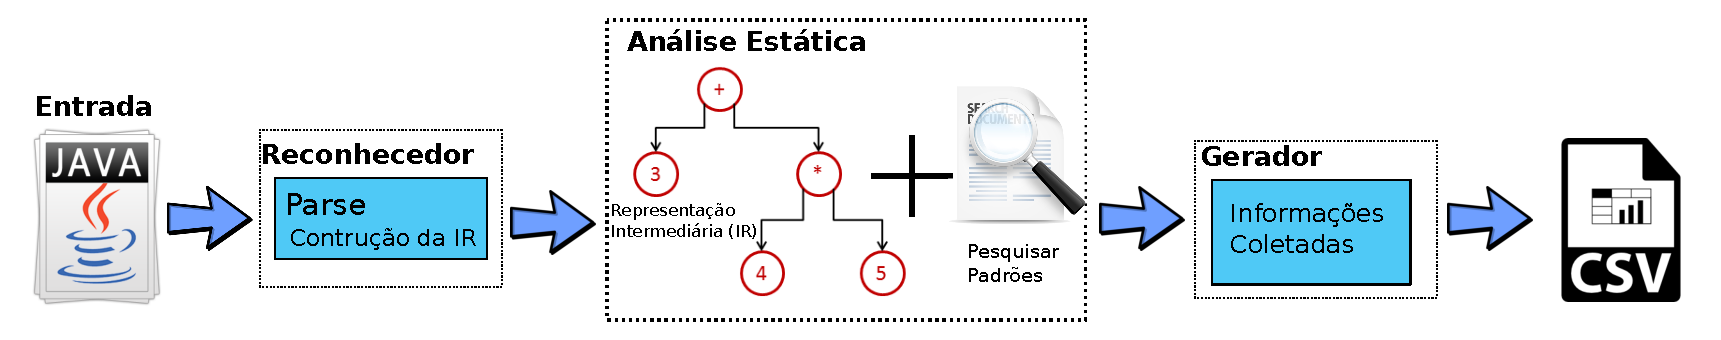
\includegraphics[scale=0.55]{Imagens/Arquitetura}
	\label{fig:Arquitetura}
	\caption{Vis\~{a}o geral da arquitetura do analisador est\'{a}tico}
\end{figure}


\section{Defini\c c\~{a}o dos Projetos a Serem Analisados}

O analisador estático recebe como entrada um arquivo \acs{CSV} (comma-separated values) 
que contém informa\c c\~{o}es sobre 
os projetos a serem analisados, como nome do projeto, 
caminho absoluto para uma pasta no sistema 
de arquivos contendo o c\'{o}digo fonte do projeto e a quantidade de linhas de código previamente 
computadas (conforme ilustrado na Figura:~\ref{fig:Arquitetura}). 
As informações contidas no arquivo \acs{CSV} s\~{a}o processadas 
por um conjunto de classes utilitárias que percorrem os diretórios 
de um determinado projeto e seleciona todos os arquivos fonte da linguagem Java. 
Os códigos fontes Java encontrados servem ent\~{a}o como a entrada 
descrita na representa\c c\~{a}o abstrata 
do analisador est\'{a}tico (Figura:~\ref{fig:Arquitetura}). Ou seja, para cada 
projeto s\~{a}o recuperados os arquivos contendo 
c\'{o}digo fonte Java, que s\~{a}o convertidos para uma 
representa\c c\~{a}o intermedi\'{a}ria (por meio de 
um parser existente); processados e analisados com 
uma infraestrutura de \emph{visitors}, e os resultados das an\'{a}lises s\~{a}o ,por fim, 
exportados.

Conforme mencionado, essa fase do analisador est\'{a}tico realiza o processamento 
de cada arquivo Java dos projetos analisados. Sob a perspectiva de usabilidade, 
o usu\'{a}rio deve executar o programa principal informando, na linha de 
comando, o caminho para o arquivo \acs{CSV} contendo as defini\c c\~{o}es dos 
projetos. Isso produz uma lista contendo todos os projetos a serem processados 
(ver Linha 25 na Figura~\ref{fig:programaPrincipal}). Ap\'{o}s a lista de 
projetos ter sido carregada, cada projeto \'{e} analisado com o uso 
da classe \texttt{ProjectAnalyser}, que possui um m\'{e}todo 
(\texttt{analyse}) com a l\'{o}gica necess\'{a}ria para 
processar a base de c\'{o}digo fonte de cada projeto. A Figure~\ref{fig:metodoAnalyse} 
apresenta a implementa\c c\~{a}o do m\'{e}todo \texttt{analyse}, que 
recebe como par\^{a}metro um projeto. Note na linha seis da 
Figura~\ref{fig:metodoAnalyse} que o resultado do \textit{parse} 
em um arquivo fonte produz uma insta\^{a}ncia da classe 
\texttt{CompilationUnit} que pertence a plataforma 
Eclipse JDT e que representa a AST de um determinado 
arquivo Java. Essa classe possui um m\'{e}todo \texttt{accept}, 
conforme o padr\~{a}o de projeto \textit{visitor}, que \'{e} usado 
para pela ferramenta de an\'{a}lise est\'{a}tica para 
coletar as informa\c c\~{o}es do uso de constru\c c\~{o}es 
Java por meio de uma an\'{a}lise da representa\c c\~{a}o 
intermedi\'{a}ria. Isso \'{e} feito considerando cada um dos 
\emph{visitors} aplicados em uma an\'{a}lise espec\'{i}fica. 
  

\begin{figure}[htb]
\begin{lstlisting}
public class Main {
   
  public static void main(String[] args) {
    
    String pathCsv = ``''; 
    
    if(args.length == 1) {
      System.out.println(``Args: ''+ args[0].toString());
      pathCsv = args[0];
    }else {
      System.out.println(``Error: inform a valid csv file!!!\nEXIT'');
      System.exit(0);
    }
    
    ReadCsv rcsv = new ReadCsv(pathCsv);
    
    List<String> errors = rcsv.getError();
    
    errors.forEach(e -> System.out.println(``Error in '' + e));
 
    ApplicationContext ctx = CDI.Instance().getContextCdi(); 
    
    ProjectAnalyser pa = ctx.getBean(``pa'', ProjectAnalyser.class);
    
    List<Project> projects = rcsv.readInput();
    
    try {
      projects.stream().forEach(project -> pa.analyse(project));
    }catch(Exception t) {
      t.printStackTrace();
    }  
  }
}
\end{lstlisting}
  \caption{Classe que representa o programa principal do analisador est\'{a}tico}
  \label{fig:programaPrincipal}
\end{figure}


\begin{figure}[htb]
\begin{lstlisting}[language=Java]
public void analyse(Project p)  {
  CompilationUnit compilationUnit = null;
  List<String> fs = IO.list(p.getPath(), new String[] { ``java'' });
    
  for (String file : fs) {
    compilationUnit = Parser.Instance().parse(new File(file));
    
    for(IVisitor visitor : listVisitors){
      visitor.getCollectedData().setProject(p);
      visitor.setFile(file);
      visitor.setUnit(compilationUnit);
        
      compilationUnit.accept((ASTVisitor) visitor);
    }
  }    
  exportData();    
}
\end{lstlisting}
 \label{fig:metodoAnalyse}
 \caption{Implementa\c c\~{a}o do m\'{e}todo \texttt{analyse}, na classe \texttt{ProjectAnalyser}.}
\end{figure}

%% \begin{figure}[h]
%% 	\center
%% 	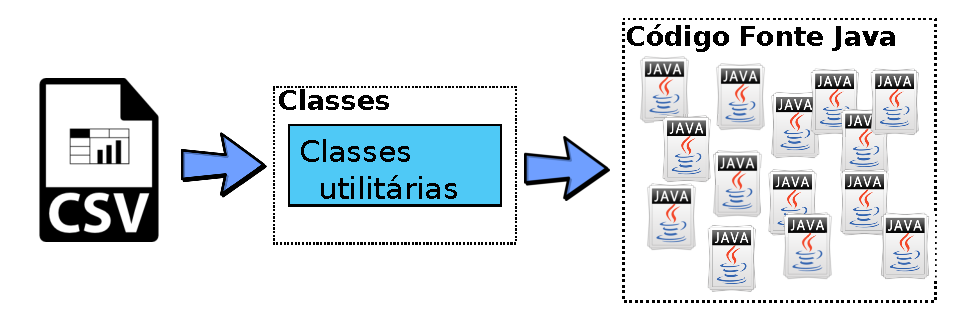
\includegraphics[scale=0.53]{Imagens/InputArquitetura}
%% 	\label{fig:InputArquitetura}
%% 	\caption{Input analisador estático.}
%% \end{figure}


\section{Análise da Representa\c c\~{a}o Intermedi\'{a}ria}

Conforme mencionado na se\c c\~{a}o anterior, o resultado do 
\textit{parser} em um arquivo fonte produz uma inst\^{a}ncia 
da classe \texttt{CompilationUnit}, que corresponde a 
uma AST com todas as defini\c c\~{o}es de tipo e 
implementa\c c\~{a}o de comportamento presentes em um m\'{o}dulo 
Java. A plataforma Eclipse JDT oferece uma infraestrutura 
de classes para realizar a traversia em uma AST, usando 
o padr\~{a}o de projeto \textit{visitor}. Dessa forma, 
foi feita uma implementa\c c\~{a}o de biblioteca de 
\textit{visitors}, para extrair as informa\c c\~{o}es 
presentes na representa\c c\~{a}o intermedi\'{a}ria.   

%% Após todos os código fontes Java identificado é dado início a verificação destes arquivos onde são processados e gerado um \textit{parser} para que os \textit{visitors} pesquisam padrões previamente estabelecidos onde a pesquisa elaborada com o principal objetivo de reconhecer elementos e sua subestruturas contidos no código fonte.
%% Com isso a representação intermediária deste analisador é o processamento do código fonte para convertê-lo em um \textit{parser} para que os  \textit{visitor} realizem sua pesquisa. A Figura:~\ref{fig:FuncionamentoAnalisador} demonstra o mais alto nível do funcionamento deste projeto.

%% \begin{figure}[h]
%% 	\center
%% 	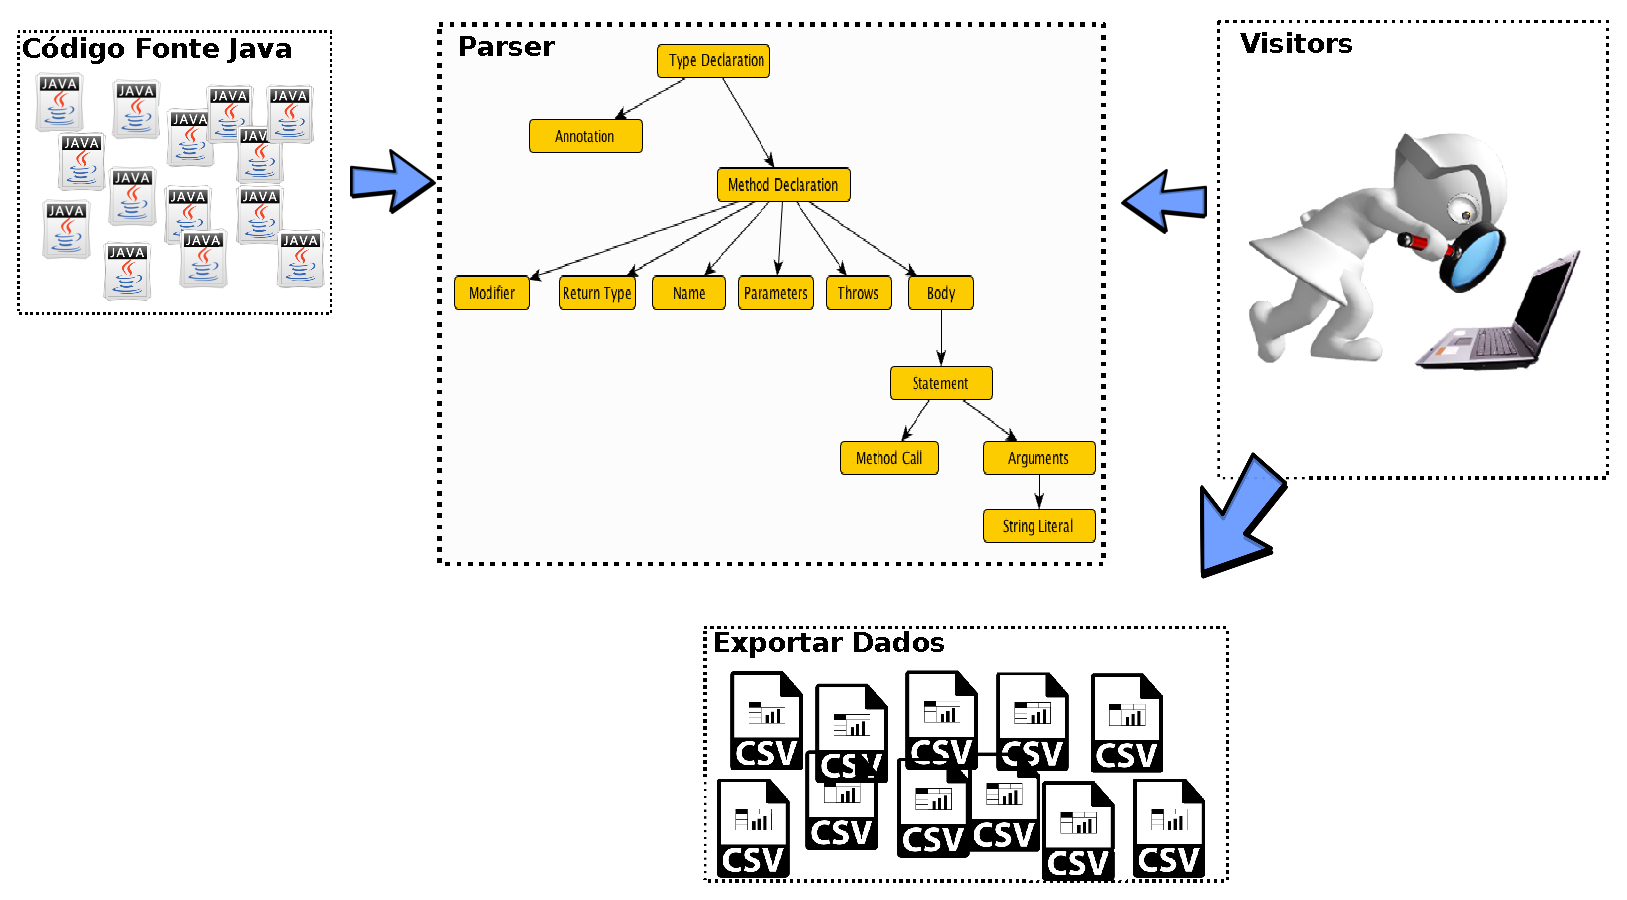
\includegraphics[scale=0.5]{Imagens/FuncionamentoVisitor}
%% 	\label{fig:FuncionamentoAnalisador}
%% 	\caption{Funcionamento analisador estático.}
%% \end{figure}

%{\color{red}{\bf rbonifacio}parece que ocorre uma transi\c c\~{a}o muito abrupta de uma discussão alto nivel para uma discussão muito rica em detalhes.}

% De forma mais técnica, a representa\c c\~{a}o intermedi\'{a}ria, para cada arquivo fonte o analisador
% est\'{a}tico realiza a coleta de dados utilizando uma infraestrutura de \textit{visitors}. 

No contexto deste projeto, 
e objetivando um maior grau de reuso, 
toda classe \emph{visitor} precisa herdar de uma classe abstrata e 
parametrizada em rela\c c\~{a}o a um tipo \texttt{T}, 
a classe \texttt{Visitor<T>}, 
onde o tipo \texttt{T} deve corresponder a classe usada para armazenar 
as informações coletadas pelo \emph{visitor}. O parâmetro de tipo \texttt{T} 
faz referência a uma 
classe composta basicamente por atributos e por 
opera\c c\~{o}es de acesso (\textit{getters} e \textit{setters}), 
que serve para representar os dados extraídos. 
Em geral, de acordo com a arquitetura do analisador est\'{a}tico proposto, 
para cada constru\c c\~{a}o que se 
deseja identificar o perfil de ado\c c\~{a}o nos projetos, s\~{a}o criadas 
duas classes: uma classe (\texttt{public class C\{ \ldots \}}) 
que representar as informa\c c\~{o}es de interesse 
associadas ao uso de uma constru\c c\~{a}o da 
linguagem Java e uma classe (\texttt{public class ConstVisitor extends Visitor<C> \{ \ldots \}}) 
que \emph{visita} a constru\c c\~{a}o de interesse na \'{a}rvore sint\'{a}tica abstrata. 
Por exemplo, a Figura~\ref{fig:enum} apresenta 
o c\'{o}digo necess\'{a}rio para visitar e popular informa\c c\~{o}es relacionadas a declara\c c\~{a}o de 
enumera\c c\~{o}es. A classe \texttt{public class Visitor<T> \{ \ldots \}} possui uma cole\c c\~{a}o 
de objetos do tipo parametrizado, sendo poss\'{i}vel adicionar inst\^{a}ncias desses objetos com a chamada 
\texttt{collectedData.addValue()}. Note que o exemplo apresentado corresponde a um dos mais simples 
\emph{visitors} implementados. Outros \emph{visitors} possuem uma l\'{o}gica mais elaborada, como por exemplo os 
\emph{visitors} que identificam oportunidades para usar constru\c c\~{o}es 
como \emph{multi-catch} ou \emph{lambda expressions}. 

\begin{figure}[htb]
\begin{lstlisting}
public class EnumDeclaration {
  private String file;
  private int startLine;
  private int endLine;
	
  //constructor + getters and setters.
}

public class EnumDeclarationVisitor extends Visitor<EnumDeclaration> {

  @Override
  public boolean visit(org.eclipse.jdt.core.dom.EnumDeclaration node) {
    
    EnumDeclaration dec = new EnumDeclaration(...);
		
    collectedData.addValue(dec);

    return true;
  }

}
\end{lstlisting}
\label{fig:enum}
\caption{Classes usadas para capturar declara\c c\~{o}es de enumera\c c\~{o}es.}
\end{figure}


%% O diagrama da Figura:~\ref*{fig:DiagramaVisitor} 
%% exibe de maneira técnica o procedimento de criar um \textit{Visitor} que detecte e colete informações dos tipos declarados no sistema, basta criar uma classes modelo \textit{TypeDeclaration.java} e  setar o parâmetro \textbf{<T>} como \textit{<TypeDeclaration>}, com isso os dados serão extraídas pelo \textit{Visitor, TypeDeclarationVisitor.java}, que identifica as informações pertinentes. {\color{red}refletir se esse par\'{a}grafo eh necessário}

%% \begin{figure}[h]
%% 	\center
%% 	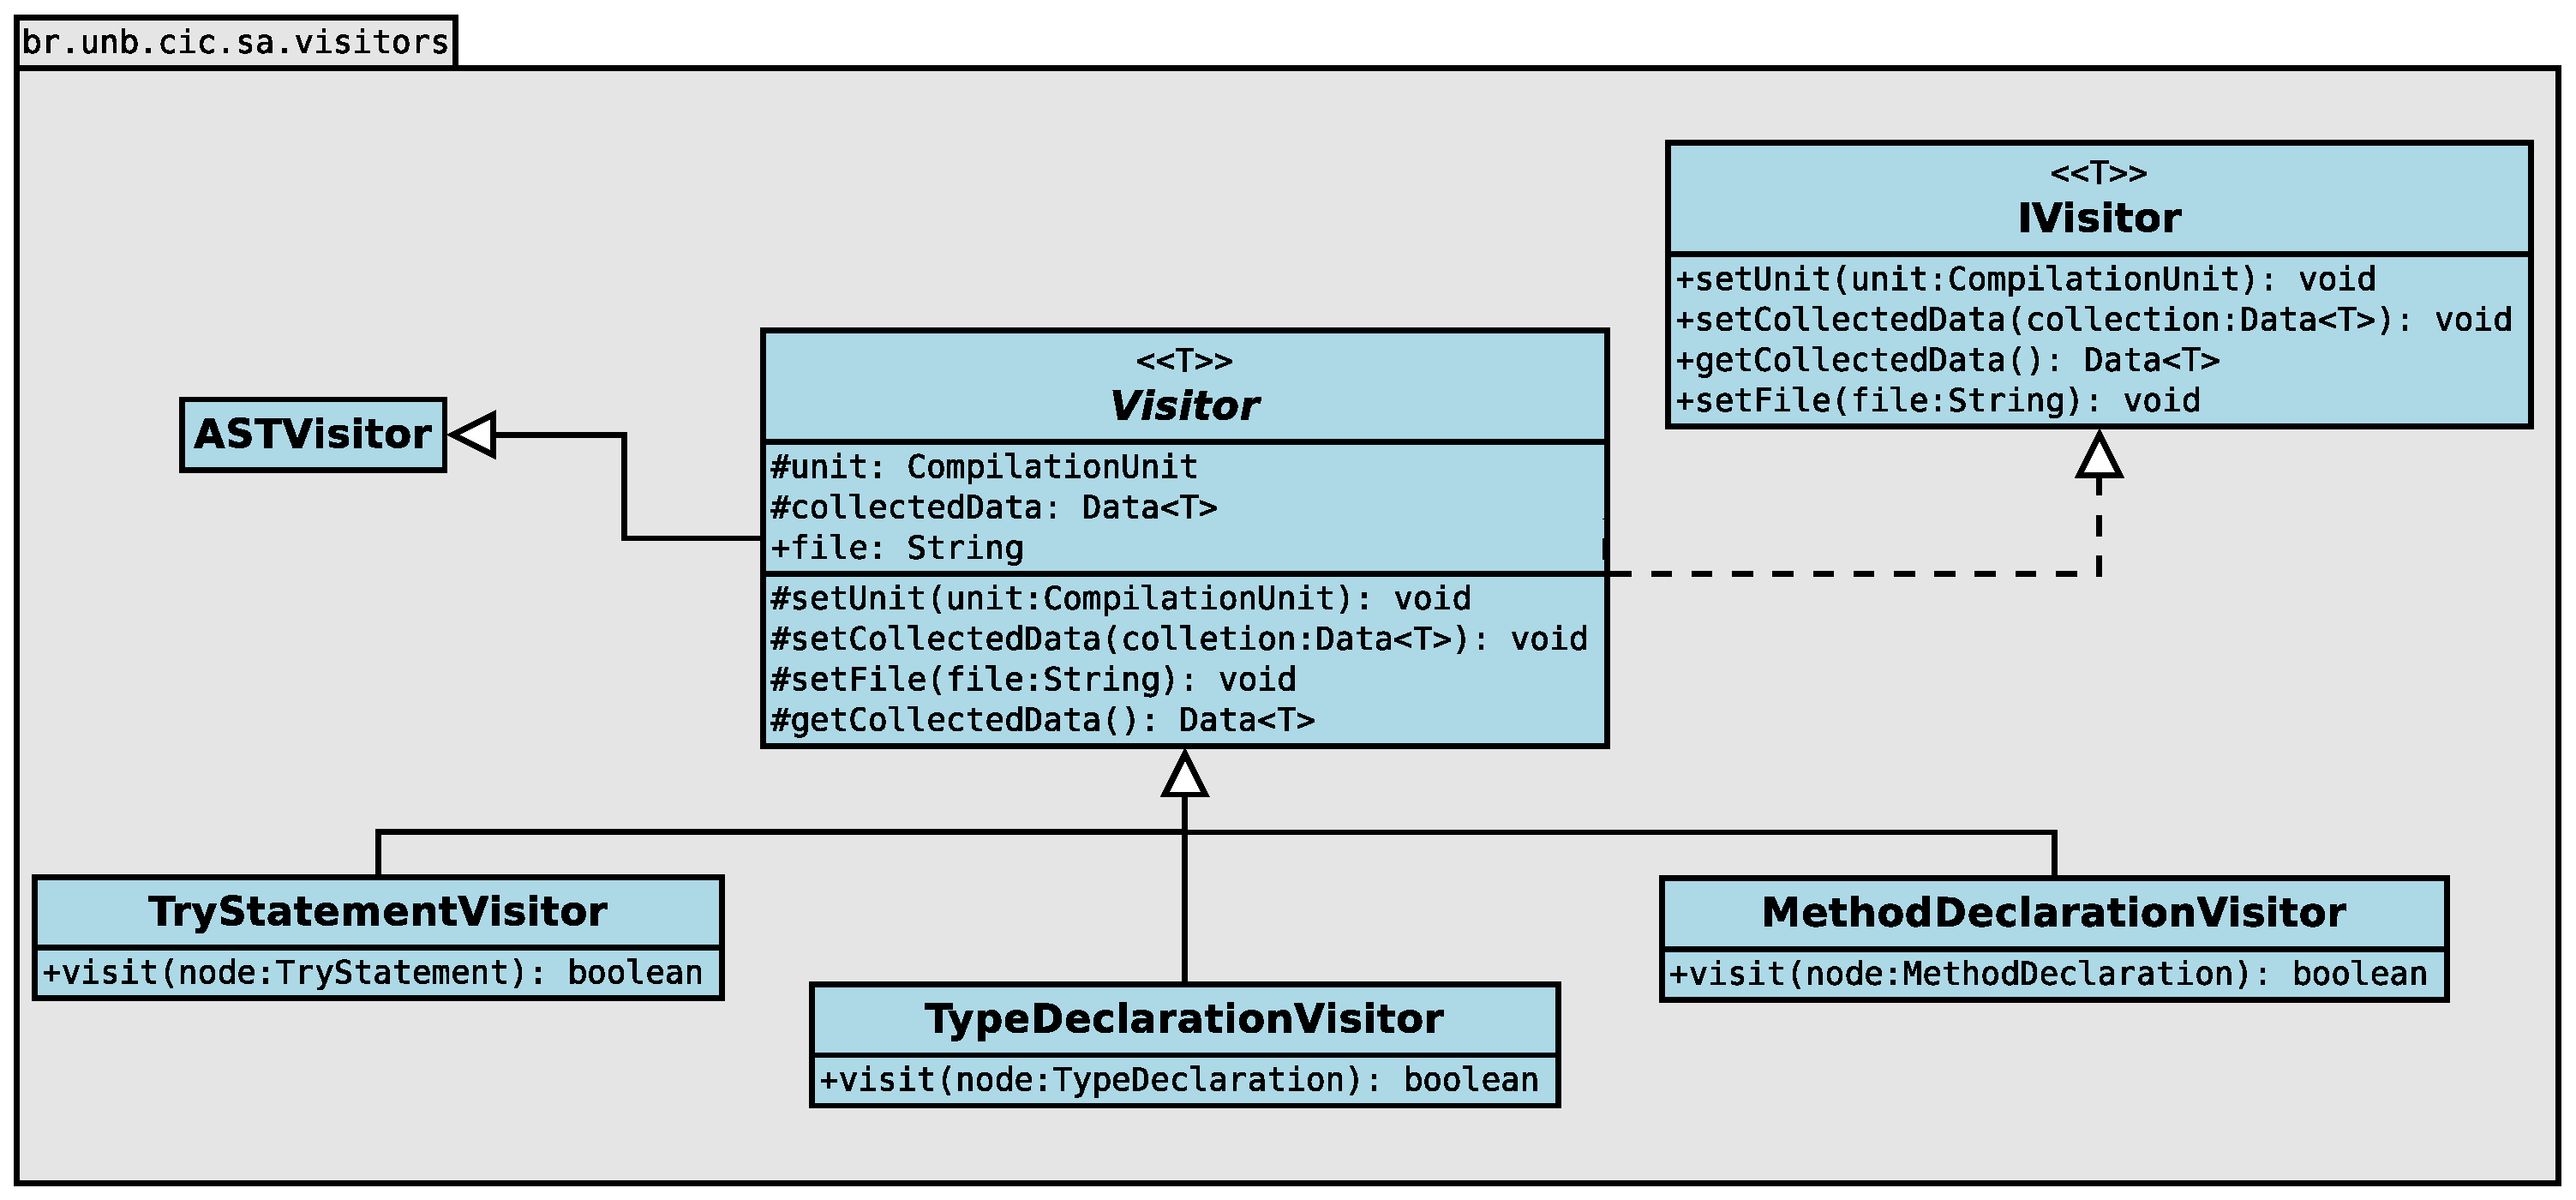
\includegraphics[scale=0.25]{Imagens/diagramaVisitor}
%% 	\label{fig:DiagramaVisitor}
%% 	\caption{Funcionamento analisador estático.}
%% \end{figure}

\subsection{Descri\c c\~{a}o dos Visitors}
Os \textit{visitors} implementados neste projeto 
s\~{a}o brevemente descritos a seguir, enquanto que 
a Tabela~\ref{tab:VisitorsCriados} apresenta 
duas m\'{e}tricas relacionadas \`{a} complexidade 
de implementa\c c\~{a}o, em termos de 
complexidade ciclom\'{a}tica e total de linhas de c\'{o}digo fonte. 
A complexidade ciclomática é dada pela quantidade de caminhos independentes 
em um trecho de código, enquanto que a quantidade de linhas de c\'{o}digo 
foi computada ignorando coment\'{a}rios e linhas em branco.  Vale 
ressaltar que a complexidade ciclom\'{a}tica 
dos \textit{visitors} varia entre um e oito  (com a média igual a 2.5). A 
quantidade média de linhas de código necessária para escrever um 
\textit{visitor} é 47.

\begin{itemize}
\item \texttt{AIC:} Coleta informa\c c\~{o}es relacionadas a declara\c c\~{a}o de 
\textit{Anonymous Inner Classes}. Tal informa\c c\~{a}o \'{e} \'{u}til 
para estimar oportunidades de uso de express\~{o}es lambda. 

\item \texttt{ExistPattern:} Coleta informa\c c\~{o}es de la\c cos \texttt{foreach} 
que iteram sobre uma cole\c c\~{a}o com o intuito de verificar se um 
determinado objeto est\'{a} presente na cole\c c\~{a}o. Tal informa\c c\~{a}o \'{e} \'{u}til 
para estimar oportunidades de uso de express\~{o}es lambda. 


\item \texttt{FieldAndVariableDeclaration:} Coleta informa\c c\~{o}es relacionadas 
a declara\c c\~{o}es de atributos e vari\'{a}veis, com o intuito de 
extrair informa\c c\~{o}es sobre a ado\c c\~{a}o de Java Generics. 

\item \texttt{FilterPattern:} Coleta informa\c c\~{o}es de la\c cos \texttt{foreach} 
que iteram sobre uma cole\c c\~{a}o com o intuito de 
filtrar elementos presentes na cole\c c\~{a}o. Tal informa\c c\~{a}o \'{e} \'{u}til 
para estimar oportunidades de uso de express\~{o}es lambda. 

\item \texttt{ImportDeclaration:} Coleta informa\c c\~{o}es relacionadas \`{a}
importa\c c\~{a}o de bibliotecas, sendo \'{u}til para estimar a ado\c c\~{a}o 
de bibliotecas voltadas para programa\c c\~{a}o concorrente ou integra\c c\~{a}o 
com linguagens de scripting, por exemplo. 

\item \texttt{LambdaExpression:} Coleta informa\c c\~{o}es relacionadas \`{a} 
ado\c c\~{a}o de express\~{o}es lambda. 

\item \texttt{Lock:} Verifica se os m\'{e}todos utilizam algum dos mecanismos 
de \emph{lock} suportados diretamente pela linguagem Java, como \texttt{Lock}, 
\texttt{ReentrantLock}, \texttt{ReadLock} ou \texttt{WriteLock}.

\item \texttt{MapPattern:} Coleta informa\c c\~{o}es de la\c cos \texttt{foreach} 
que iteram sobre uma cole\c c\~{a}o com o intuito de 
aplicar alguma opera\c c\~{a}o sobre os elementos presentes na cole\c c\~{a}o. 
Tal informa\c c\~{a}o \'{e} \'{u}til 
para estimar oportunidades de uso de express\~{o}es lambda. 

\item \texttt{MethodCall:} Coleta informa\c c\~{o}es relacionadas \`{a}s 
chamadas de m\'{e}todo, sendo \'{u}til para estimar o uso da API de 
introspec\c c\~{a}o de c\'{o}digo, por exemplo. 

\item \texttt{MethodDeclaration:} Coleta informa\c c\~{o}es relacionadas 
\`{a}s declara\c c\~{o}es de m\'{e}todos, sendo \'{u}til para identificar 
padr\~{o}es de uso de Java Generics, por exemplo.

\item \texttt{ScriptEngine:} Coleta informa\c c\~{o}es relacionadas 
ao uso da API Java para integra\c c\~{a}o com linguagens de scripting.  

\item \texttt{SwitchStatement:} Coleta informa\c c\~{o}es relacionadas 
ao uso de senten\c cas \texttt{switch-case}, com o intuito principal 
de identificar o uso de \texttt{strings} nesse tipo de senten\c ca. 

\item \texttt{SwitchString:} Coleta informa\c c\~{o}es associadas \`{a}s 
oportunidades de reestrutura\c c\~{a}o de c\'{o}digo para usar 
senten\c cas \texttt{switch-case} com \texttt{strings}. 

\item \texttt{TryStatement:} Coleta informa\c c\~{o}es relacionadas 
ao uso de blocos \texttt{try-catch}, em particular para estimar o 
uso da constru\c c\~{a}o \texttt{try-with-resources}. 

\item \texttt{TypeDeclaration:} Coleta informa\c c\~{o}es sobre 
os tipos declarados (classes, interfaces, enumera\c c\~{o}es), com 
o intuito, por exemplo, de estimar a ado\c c\~{a}o de Java Generics. 
\end{itemize}

\begin{table}[ht] \footnotesize
	\centering
	\caption{Estimativa da complexidade de desenvolvimento de cada \emph{visitor}.}
	\label{tab:VisitorsCriados}	
    \begin{tabular}{crr}
%		\begin{tabular}{M|p{9cm}}% centered column
			\hline 
			Visitor &  \acs{CC} & \acs{LoC}\\ \hline \hline
			
			\texttt{AIC} & 6 & 64\\ 
			
			\texttt{ExistPattern}  & 28 & 116\\ 
			
			\texttt{FieldAndVariableDeclaration} & 8 & 81\\ 
			
			\texttt{FilterPattern}  & 43 & 168\\ 
			
			\texttt{ImportDeclaration}& 1 & 63\\ 
			
			\texttt{LambdaExpression} & 1 & 33\\ 
			
			\texttt{Lock} & 12 & 75\\ 
			
			\texttt{MapPattern} & 27 & 103\\ 
			
			\texttt{MethodCall} & 2 & 22\\ 
			
			\texttt{MethodDeclaration} & 5 & 45\\ 
			
			\texttt{ScriptingEngine} & 5 & 39\\ 
			
			\texttt{SwitchStatement} & 3 & 35\\ 
			
			\texttt{SwitchStringOpportunities} & 3 & 50\\ 
		
			\texttt{TryStatement} & 11 & 80\\ 
			
			\texttt{TypeDeclaration} & 2 & 41\\ \hline
		\end{tabular}
\end{table}

% \section{Exporta\c c\~{a}o dos dados}

%% Para exportar os dados coletadas, foi constru\'{i}da uma solu\c c\~{a}o extens\'{i}vel, baseada no padr\~{a}o 
%% \emph{Inje\c c\~{a}o de Depend\^{e}ncia} e introspec\c c\~{a}o de c\'{o}digo. 
%% %\subsection{Injeçao de Dependência}


\subsection{Extensibilidade para Inclus\~{a}o de Novos Visitors}

Para tornar a solu\c c\~{a}o mais extens\'{i}vel, foram utilizados os mecanismos de 
\emph{Inje\c c\~{a}o de Depend\^{e}ncia} e introspec\c c\~{a}o de c\'{o}digo. 
Injeção de dependência \acs{DI}, \'{e} um mecanismo de extensibilidade mais 
conhecido como um padr\~{a}o de projeto originalmente denominado de inversão de controle (\acs{IoC}). 
De acordo com esse mecanismo, a sequência de criação dos objetos depende de como os mesmos são 
solicitados pelo sistema. Ou seja, quando um sistema é iniciado, 
os objetos necess\'{a}rios são instanciados e injetados de forma apropriada, 
geralmente de acordo com arquivo de configura\c c\~{o}es.
O mecanismo de inje\c c\~{a}o de depend\^{e}ncia foi incorporado na arquitetura 
com o uso do \textit{framework} Spring~\cite{SPRING_REF}, o que n\~{a}o causou 
nenhum impacto significativo na solu\c c\~{a}o inicialmente proposta e que n\~{a}o 
fazia uso de tal mecanismo os \emph{visitors} eram instanciados de maneira 
\emph{program\'{a}tica}. O uso do mecanismo de inje\c c\~{a}o de depend\^{e}ncia 
serviu para flexibilizar n\~{a}o apenas a incorpora\c c\~{a}o de novos \emph{visitors}, 
mas tamb\'{e}m para definir, de forma mais flex\'{i}vel, a estrat\'{e}gia de exporta\c c\~{a}o dos dados 
coletados. Gra\c cas ao mecanismo de inje\c c\~{a}o de depend\^{e}ncia, o desenvolvedor pode 
concentrar seu esforço na criação de \textit{visitors}, fazendo como que estes implementem a 
l\'{o}gica necess\'{a}ria para extrair as informações. Para que novos \emph{visitors} se conectem 
a plataforma, tornou-se necess\'{a}rio declarar o \textit{visitor} no arquivo com a defini\c c\~{a}o 
dos objetos gerenciados pelo Spring~\cite{SPRING_REF}.


\section{Exporta\c c\~{a}o dos Dados}

Na vers\~{a}o atual do suporte ferramental desenvolvido nessa monografia, os dados 
coletados pelo analisador est\'{a}tico s\~{a}o exportados exclusivamente no formato 
CSV. Esse formato facilita as an\'{a}lises estat\'{i}sticas usando o ambiente e linguagem 
de programa\c c\~{a}o R~\cite{R}. Também com foco na extensibilidade do sistema, os componentes envolvidos na 
geração de relatórios utilizam os mecanismos de inje\c c\~{a}o de depend\^{e}ncia, mencionado na 
se\c c\~{a}o anterior, e introspec\c c\~{a}o de c\'{o}digo, via a a API \textit{Reflection} da linguagem de 
programa\c c\~{a}o Java. Tal mecanismo oferece aos programadores a capacidade de escreverem componentes 
que podem observar e até modificar a estrutura e o comportamento dos objetos em tempo de execução.

A geração dos relatórios utiliza a classe \texttt{public class CSVData<T> \{ \ldots \ \}} onde o 
tipo parametrizado \texttt{<T>} é o mesmo utilizado para representar 
os dados coletados pelos \textit{visitors}. 
Os dados são obtidos através dos métodos de acesso (\textit{getters}) destas 
classes e exportados para arquivos~\acs{CSV}. 
O método \textit{export()} da classe \textbf{CSVData<T>} descobre quais dados s\~{a}o armazenados nos objetos do 
tipo \textbf{<T>}, usando o mecanismo de introspec\c c\~{a}o de c\'{o}digo. Com isso, \'{e} poss\'{i}vel 
generalizar a implementa\c c\~{a}o e simplificar a exporta\c c\~{a}o de dados coletados a partir de 
\textit{visitors} espec\'{i}ficos. Ou seja, após a descoberta dos dados coletados pelos \textit{visitors} usando 
introspec\c c\~{a}o, \'{e} poss\'{i}vel recuperar os mesmos assumindo a exist\^{e}ncia de m\'{e}todos de 
acesso (\textit{getters} de acordo com a especifica\c c\~{a}o Java Beans) e, 
como isso, export\'{a}-los em arquivos \acs{CSV} de saída. 
A Figura~\ref{fig:exportacao} apresenta o uso desse mecanismo para generalizar a exporta\c c\~{a}o dos 
dados. 

\begin{figure}
\begin{lstlisting}[language=Java]
public class CSVData<T> implements Data<T> {

  @Override
  public void export() {
    StringBuffer str = new StringBuffer("");
      
    if(data == null) { return; }
      
    for(T value : data) {
      //reflection code...
      for(Field f: value.getClass().getDeclaredFields()){
	  
	String fieldName = f.getName();
	String prefix = "get";
	  
	if(f.getType().isPrimitive() && f.getType().equals(Boolean.TYPE)) {
	  prefix = "is";
	}
					
	String methodName = prefix +
	Character.toUpperCase(fieldName.charAt(0)) +
	fieldName.substring(1);
	  
	Method m = value.getClass().getDeclaredMethod(methodName);						
	str.append(m.invoke(value));
	str.append(";");
	
	writer.append(str.toString());
	writer.append("\n");			
		
	writer.flush();  
      }
    }
  }
\end{lstlisting}
\label{fig:exportacao}
\caption{Exporta\c c\~{a}o de dados usando o mecanismo de introspec\c c\~{a}o de c\'{o}digo.}
\end{figure}

%Projetar um analisador estático para extrair informações de softwares desenvolvido não é uma simples tarefa, entretanto EclipseJDT~\cite{EclipseJDT} prove uma abstração significativa tornado menos árdua este projeto. O que pode possibilitar projetar uma arquitetura mais robusta para este analisador onde o foco de qualquer desenvolvedor que deseje utilizá-lo concentre-se apenas na produção de seus \textit{Visitors}. 
%
%Um ponto de extrema relevância foi tornar este analisador independente de qualquer plataforma e \acs{IDE} foi um ponto vital para o concepção deste projeto que não tem como intuito ser plugin de qualquer \acs{IDE} o que acarretaria na limitação do seu uso a um cenário específico mas sim uma ferramenta para apoiar no desenvolvimento de um software com construções atuais. Utilizando a portabilidade nativa entre as plataformas provido pela linguagem Java este trabalho foi concebido com intuito de atender ao mais diversos desenvolvedores quer utilizem Linux, Windows, Mac ou qualquer outro sistema operacional que tenha suporte para Java.
%
%A análise tem como início a seleção de projetos, nesse caso seleção em repositórios públicos, onde após o download é informado analisador o diretório raiz onde estes estão localizados. Após é iniciado uma listagem dos arquivos fonte Java contidos nos projeto e contabilizados o total de \acs{LOC} e criado uma árvore sintática para cada arquivo encontrado através de um \textit{parser} provido pela biblioteca EclipseJDT~\cite{EclipseJDT}. Em seguida os \textit{Visitors} são instanciados com o objetivo de percorrer os nós destas árvores para pesquisar por construções de código previamente determinadas.
%
%Todas as construções pesquisadas quando encontradas pelos \textit{Visitors} são armazenadas temporariamente enquanto o analisador verifica todo projeto, quando é verificado a última árvore sintática pelos \textit{Visitors} é iniciado o processo de exportar os dados encontrados para um arquivo \acs{CSV} o conteúdo relevante destes blocos, a Figura:~\ref{fig:Arquitetura} demostra de maneira clara o funcionamento do analisador. Após a exportação dos dados o analisador inicia todo processo novamente caso exista mais de um projeto.
%
%Devido ao mecanismo de \textit{reflection} proveniente da linguagem Java, o desenvolvedor não tem a necessidade de implementar código para exportação de dados tendo em vista que isto ocorre automaticamente através da introspecção realizada pelo analisador extraindo os dados armazenados pelos \textit{Visitors}.

%	\begin{figure}[h]
%		\center
%		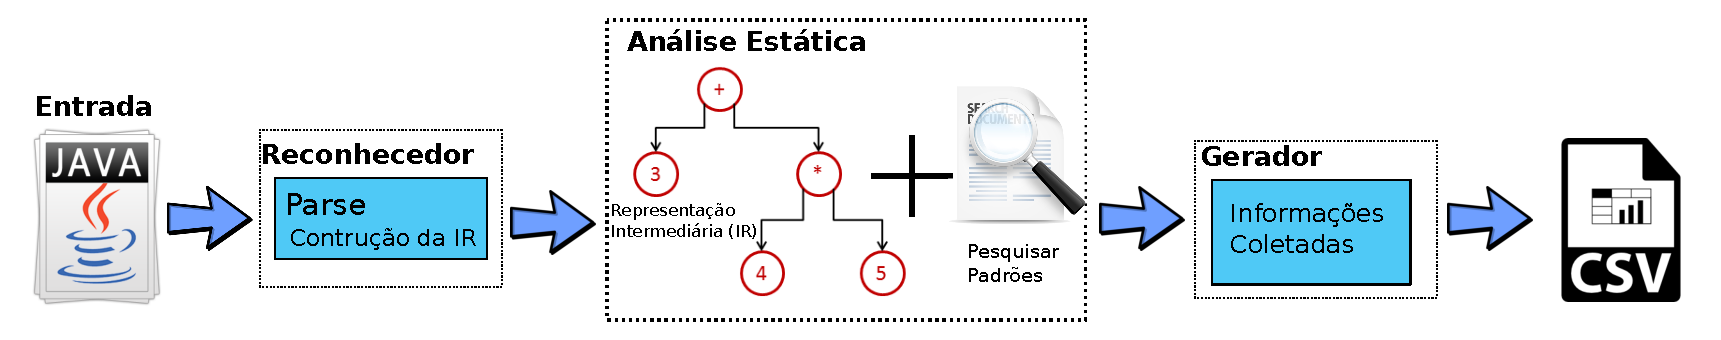
\includegraphics[scale=0.52]{Imagens/Arquitetura}
%		\label{fig:Arquitetura}
%		\caption{Funcionamento analisador estático.}
%	\end{figure}


%\section{Arquitetura}
%
%\subsection{Visitors}
%
%
%
%\begin{lstlisting}
%package br.unb.cic.sa.visitors;
%
%import org.eclipse.jdt.core.dom.ASTVisitor;
%import org.eclipse.jdt.core.dom.CompilationUnit;
%import br.unb.cic.sa.model.Data;
%
%public class Visitor<T> extends ASTVisitor implements IVisitor<T> {
%	protected CompilationUnit unit;
%	protected Data<T> collectedData;
%	protected String file;
%	
%	public Visitor() {}
%	
%	@Override
%	public void setUnit(CompilationUnit unit) { this.unit = unit; }
%	
%	@Override
%	public void setCollectedData(Data<T> colletion) { this.collectedData = colletion; }
%	
%	@Override
%	public void setFile(String file) {	this.file = file; }
%
%	@Override
%	public Data<T> getCollectedData() {	return collectedData;	}	
%}
%\end{lstlisting}
%
%
%A tabela:~\ref{tab:VisitorsCriados} detalha os 17 \textit{Visitors} criados com a respectiva descrição do trabalho realizado. Como forma de exemplificar a criação de um \textit{Visitors}, etapa a qual é composta de 4 passos quo serão demonstrados a seguir.
%
%A investigação para saber como o tratamento de exceção Java tem sido utilizado acarretou na criação de um \textit{Visitor} específico para este fim, \textit{TryStatementVisitor}, responsável por pesquisar este mecanismo o qual pode contar com alguma evoluções ao logo do histórico da linguagem Java. A pesquisa é iniciada encontrando blocos \textit{trys/catch}, onde destes será coletadas as informações referentes a adoção de \textit{resources} e oportunidade de utilizar \textit{multicatch} em blocos \textit{trys} que contenham \textit{catchs} iguais aninhados.
%%, neste caso de oportunidades os \textit{catchs} são testados por igualdade mas é trivial a utilização de um algoritmo mais avançado que teste a similaridade.
%
%Criação do \textit{Visitor TryStatementVisitor} com exemplo.
%
%	\begin{enumerate}
%		\item Inicialmente é necessário criar a classe modelo onde esta terá atribuição de receber os dados que serão extraídos pelos \textit{Visitors}, basicamente as classes modelos são compostas de \textit{getters} e \textit{setters} e são declaradas no pacote  \textit{\textbf{br.unb.cic.sa.model}}.
%			\begin{lstlisting}
%package br.unb.cic.sa.model;
%
%public class TryStatementData  {
%	private String file;
%	private int startLine;
%	private int endLine;
%	private boolean tryWithResource = false;
%	private boolean multiCatch = false;
%	
%	public TryStatementData(String file, int startLine, int endLine){
%		this.file = file;
%		this.startLine = startLine;
%		this.endLine = endLine;
%	}
%	
%	//getters and setters
%}
%			\end{lstlisting}
%			
%			
%		\item Em seguida, é concebida a criação do \textit{Visitor} no pacote \textit{\textbf{br.unb.cic.sa.visitors}} onde esta nova classe será estendida da classe parametrizada \textit{\textbf{Visitor<TryStatementData>}} apresentada anteriormente onde a parametrização desta classe é o modelo criado anteriormente.
%			
%			\begin{lstlisting}
%package br.unb.cic.sa.visitors;
%
%import java.util.List;
%import org.eclipse.jdt.core.dom.CatchClause;
%import org.eclipse.jdt.core.dom.TryStatement;
%import br.unb.cic.sa.model.TryStatementData;
%import br.unb.cic.sa.similarity.BasicSimilarityChecker;
%import br.unb.cic.sa.similarity.SimilarityChecker;
%
%public class TryStatementVisitor extends Visitor<TryStatementData> {
%
%	SimilarityChecker similarity;
%
%	public TryStatementVisitor() {
%		similarity = new BasicSimilarityChecker();
%	}
%
%	@Override
%	public boolean visit(s node) {
%
%		TryStatementData t = new TryStatementData(this.file, unit.getLineNumber(node.getStartPosition()),
%				unit.getLineNumber(node.getStartPosition() + node.getLength()));
%		
%		if (node.resources().size() > 0) {
%			t.setTryWithResource(true);
%		}
%	
%		if (node.catchClauses().size() > 1) {
%			if (this.checkSimilarity(node.catchClauses())) {
%				t.setMultiCatch(true);
%			}
%		}
%
%		this.collectedData.addValue(t);
%
%		return super.visit(node);
%	}
%	
%	private boolean checkSimilarity(List<CatchClause> catchClause) {
%		for (CatchClause cc : catchClause) {
%			for (CatchClause cn : catchClause) {
%				// To ignore the same catch in loops
%				if (!cc.equals(cn)) {
%				
%				//Chamada externa para testar similaridade
%					if (this.similarity.checkSimilarity(cc.getBody(),
%														cn.getBody())) {
%						return true;
%					}
%				}
%			}
%		}
%		return false;
%	}
%
%}
%			\end{lstlisting}
%			
%		 Na linha24, é testada a condição para saber se este bloco fez adoção de \textit{Resouce}. Na linha 30 é verificado que o bloco é um possível caso de \textit{multicatch} pois existe mais de um bloco. Na linha 39 tem-se o método \textit{checkSimilarity} o qual efetua a comparação dos blocos \textit{Catch} aninhados, entretando de forma trivial na linha 46, pode ser utilizado um algoritmo mais sofisticado para testar por similaridade modificando apenas o conteúdo do método \textbf{\textit{checkSimilarity}} da classe \textit{\textbf{SimilarityChecker}} o que não resulta em mudanças neste \textit{Visitor}.
%		
%	
%			\item Em seguida deve-se declarar o cabeçalho no arquivo \textit{resource/Beans.xml} do \textit{Spring} que estará presente no \acs{CSV} de saída. Onde este cabeçalho é composto pelo dados que serão extraídos pelos \textit{Visitors} e armazenados no modelo criado.
%			
%			\begin{lstlisting}
%<bean id="tryStatementData" class="br.unb.cic.sa.model.CSVData">
%	<property name="outDir" value="output"/>
%	<property name="fileName" value="tryStatement"/>
%	<property name="head" value="typeProject, before, project, version, file, start, end, resource, multiCatch"/> 
%</bean>
%			\end{lstlisting}
%			
%			
%			\item Por fim declarar o \textit{Visitor} como um \textit{bean} do \textit{Spring} para que este seja injetado no projeto e assim realize sua pesquisa.
%			
%			\begin{lstlisting}
%<bean id="tryStatementVisitor" class="br.unb.cic.sa.visitors.TryStatementVisitor">
%	<property name="collectedData" ref="tryStatementData"/>
%</bean>
%			\end{lstlisting}
%			
%	\end{enumerate}
%
%
%
%\subsection{Exportar Dados}
%A exportação dos dados para \acs{CSV} é realizado de forma automática utilizando o mecanismo de \textit{reflection} fornecido por Java. A classe parametrizada \textbf{\textit{CSVData<T>}} no pacote \textbf{\textit{br.unb.cic.sa.model}} implementa a interface \textit{\textbf{Data<T>}} onde \textbf{\textit{<T>}} faz  aos modelos declarados para as informações coletadas.
%
%\begin{lstlisting}
%package br.unb.cic.sa.model;
%
%public interface Data<T> {
%	public void setProject(Project project);
%	public void addValue(T value);
%	public void export();
%	public int size();
%	public void clean();
%}
%\end{lstlisting}
%
%
%Onde o atributo \textit{String[] head} é injetado pelo \textit{Spring} pois fora declarado anteriormente na criação do visitor. O método \textbf\textit{{export()}}, na linha 23, é o método responsável para exportar os dados em seus respectivos \acs{CSV} pois este método recupera as informações contidas nas coleções populadas pelos \textit{Visitors} e com \textit{reflection} captura os campos declarados em especial para os métodos quais são pré-fixados com \textit{get ou is} que terão seus valores capturados para que sejam exportados.
%
%\begin{lstlisting}
%package br.unb.cic.sa.model;
%
%import java.io.File;
%import java.io.FileWriter;
%import java.io.IOException;
%import java.lang.reflect.Field;
%import java.lang.reflect.InvocationTargetException;
%import java.lang.reflect.Method;
%import java.util.ArrayList;
%import java.util.List;
%
%public class CSVData<T> implements Data<T>{
%
%	private Project project;
%	private String fileName;
%	private String outDir;
%	private String[] head; 
%	private List<T> data;
%
%	...
%	
%	@Override
%	public void export() {
%		
%		try (FileWriter writer = new FileWriter(this.makeCsv(head), true)){
%		
%			StringBuffer str = new StringBuffer("");
%
%			if(data == null) {
%				return;
%			}
%			
%			for(T value : data) {
%				str = new StringBuffer("");
%				
%				str.append(project.getTypeOfProject());
%				str.append(";");
%				str.append(project.getBefore());
%				str.append(";");
%				str.append(project.getProjectName());
%				str.append(";");
%				str.append(project.getProjectRevision());
%				str.append(";");
%			
%				for(Field f: value.getClass().getDeclaredFields()){
%										
%					String fieldName = f.getName();
%					String prefix = "get";
%					
%					if(f.getType().isPrimitive() &&
%					   f.getType().equals(Boolean.TYPE)) {
%						prefix = "is";
%					}
%					
%					String methodName = prefix + 
%								Character.toUpperCase(fieldName.charAt(0)) +
%								fieldName.substring(1);
%										
%					try {
%						Method m = value.getClass().getDeclaredMethod(methodName);						
%						str.append(m.invoke(value));
%						str.append(";");
%					}catch(
%							NoSuchMethodException | 
%							IllegalAccessException |
%							IllegalArgumentException |
%							InvocationTargetException e) {
%							
%						throw new RuntimeException("Type " + 
%											value.getClass().getName() +
%											" must have a method named " +
%											 methodName);
%					}
%				}
%				
%				writer.append(str.toString());
%				writer.append("\n");
%				
%			}
%		
%			writer.flush();
%		
%		}
%		catch(Exception e) {
%			e.printStackTrace();
%		}
%	}
%}
%
%\end{lstlisting}
